\documentclass[]{bilingualworkshop}

% latex file for the aberystwyth university magician chassis programming workshop
%
% set engtrue to print the english version
% set cymtrue to print the welsh version

\engtrue  %english version
%\cymtrue   %cymraeg version
  
\wsversion{1.2} % version


\aulogo{
\includegraphics[width=0.3\textwidth]{logo.png}} % Institution logo at the top right of the memo, comment out this line for no logo
\footerLogoOne{
\includegraphics[height=0.08\textwidth]{img/arc.png}}
%\footerLogoTwo{\includegraphics[height=0.08\textwidth]{img/playful-coding.png}}
%\footerLogoThree{
\includegraphics[height=0.08\textwidth]{img/arc.png}}
%\footerLogoFour{\includegraphics[height=0.08\textwidth]{img/playful-coding.png}}
%\footerLogoFive{
\includegraphics[height=0.08\textwidth]{img/arc.png}}

  \title{\en{Aberystwyth Robotics Club - Magician Chassis - Programming Instructions}\cy{Teitl Cymraeg}}
  
   	\usepackage{listings}
    \usepackage{wrapfig}
    \usepackage{caption}
    %%%%%%%%%%%%%%%%%%%%%%%%%%%%%%%%%%%%%%%%%%%%%%%%%%%%%%%%%%%%%%%%%%%%%%%%%%%%%%%% 
%%% ~ Arduino Language - Arduino IDE Colors ~                                  %%%
%%%                                                                            %%%
%%% Kyle Rocha-Brownell | 10/2/2017 | No Licence                               %%%
%%% -------------------------------------------------------------------------- %%%
%%%                                                                            %%%
%%% Place this file in your working directory (next to the latex file you're   %%%
%%% working on).  To add it to your project, place:                            %%%
%%%    %%%%%%%%%%%%%%%%%%%%%%%%%%%%%%%%%%%%%%%%%%%%%%%%%%%%%%%%%%%%%%%%%%%%%%%%%%%%%%%% 
%%% ~ Arduino Language - Arduino IDE Colors ~                                  %%%
%%%                                                                            %%%
%%% Kyle Rocha-Brownell | 10/2/2017 | No Licence                               %%%
%%% -------------------------------------------------------------------------- %%%
%%%                                                                            %%%
%%% Place this file in your working directory (next to the latex file you're   %%%
%%% working on).  To add it to your project, place:                            %%%
%%%    %%%%%%%%%%%%%%%%%%%%%%%%%%%%%%%%%%%%%%%%%%%%%%%%%%%%%%%%%%%%%%%%%%%%%%%%%%%%%%%% 
%%% ~ Arduino Language - Arduino IDE Colors ~                                  %%%
%%%                                                                            %%%
%%% Kyle Rocha-Brownell | 10/2/2017 | No Licence                               %%%
%%% -------------------------------------------------------------------------- %%%
%%%                                                                            %%%
%%% Place this file in your working directory (next to the latex file you're   %%%
%%% working on).  To add it to your project, place:                            %%%
%%%    \input{arduinoLanguage.tex}                                             %%%
%%% somewhere before \begin{document} in your latex file.                      %%%
%%%                                                                            %%%
%%% In your document, place your arduino code between:                         %%%
%%%   \begin{lstlisting}[language=Arduino]                                     %%%
%%% and:                                                                       %%%
%%%   \end{lstlisting}                                                         %%%
%%%                                                                            %%%
%%% Or create your own style to add non-built-in functions and variables.      %%%
%%%                                                                            %%%
 %%%%%%%%%%%%%%%%%%%%%%%%%%%%%%%%%%%%%%%%%%%%%%%%%%%%%%%%%%%%%%%%%%%%%%%%%%%%%%%% 

\usepackage{color}
\usepackage{listings}    
\usepackage{courier}

%%% Define Custom IDE Colors %%%
\definecolor{arduinoGreen}    {rgb} {0.17, 0.43, 0.01}
\definecolor{arduinoGrey}     {rgb} {0.47, 0.47, 0.33}
\definecolor{arduinoOrange}   {rgb} {0.8 , 0.4 , 0   }
\definecolor{arduinoBlue}     {rgb} {0.01, 0.61, 0.98}
\definecolor{arduinoDarkBlue} {rgb} {0.0 , 0.2 , 0.5 }

%%% Define Arduino Language %%%
\lstdefinelanguage{Arduino}{
  language=C++, % begin with default C++ settings 
%
%
  %%% Keyword Color Group 1 %%%  (called KEYWORD3 by arduino)
  keywordstyle=\color{arduinoGreen},   
  deletekeywords={  % remove all arduino keywords that might be in c++
                break, case, override, final, continue, default, do, else, for, 
                if, return, goto, switch, throw, try, while, setup, loop, export, 
                not, or, and, xor, include, define, elif, else, error, if, ifdef, 
                ifndef, pragma, warning,
                HIGH, LOW, INPUT, INPUT_PULLUP, OUTPUT, DEC, BIN, HEX, OCT, PI, 
                HALF_PI, TWO_PI, LSBFIRST, MSBFIRST, CHANGE, FALLING, RISING, 
                DEFAULT, EXTERNAL, INTERNAL, INTERNAL1V1, INTERNAL2V56, LED_BUILTIN, 
                LED_BUILTIN_RX, LED_BUILTIN_TX, DIGITAL_MESSAGE, FIRMATA_STRING, 
                ANALOG_MESSAGE, REPORT_DIGITAL, REPORT_ANALOG, SET_PIN_MODE, 
                SYSTEM_RESET, SYSEX_START, auto, int8_t, int16_t, int32_t, int64_t, 
                uint8_t, uint16_t, uint32_t, uint64_t, char16_t, char32_t, operator, 
                enum, delete, bool, boolean, byte, char, const, false, float, double, 
                null, NULL, int, long, new, private, protected, public, short, 
                signed, static, volatile, String, void, true, unsigned, word, array, 
                sizeof, dynamic_cast, typedef, const_cast, struct, static_cast, union, 
                friend, extern, class, reinterpret_cast, register, explicit, inline, 
                _Bool, complex, _Complex, _Imaginary, atomic_bool, atomic_char, 
                atomic_schar, atomic_uchar, atomic_short, atomic_ushort, atomic_int, 
                atomic_uint, atomic_long, atomic_ulong, atomic_llong, atomic_ullong, 
                virtual, PROGMEM,
                Serial, Serial1, Serial2, Serial3, SerialUSB, Keyboard, Mouse,
                abs, acos, asin, atan, atan2, ceil, constrain, cos, degrees, exp, 
                floor, log, map, max, min, radians, random, randomSeed, round, sin, 
                sq, sqrt, tan, pow, bitRead, bitWrite, bitSet, bitClear, bit, 
                highByte, lowByte, analogReference, analogRead, 
                analogReadResolution, analogWrite, analogWriteResolution, 
                attachInterrupt, detachInterrupt, digitalPinToInterrupt, delay, 
                delayMicroseconds, digitalWrite, digitalRead, interrupts, millis, 
                micros, noInterrupts, noTone, pinMode, pulseIn, pulseInLong, shiftIn, 
                shiftOut, tone, yield, Stream, begin, end, peek, read, print, 
                println, available, availableForWrite, flush, setTimeout, find, 
                findUntil, parseInt, parseFloat, readBytes, readBytesUntil, readString, 
                readStringUntil, trim, toUpperCase, toLowerCase, charAt, compareTo, 
                concat, endsWith, startsWith, equals, equalsIgnoreCase, getBytes, 
                indexOf, lastIndexOf, length, replace, setCharAt, substring, 
                toCharArray, toInt, press, release, releaseAll, accept, click, move, 
                isPressed, isAlphaNumeric, isAlpha, isAscii, isWhitespace, isControl, 
                isDigit, isGraph, isLowerCase, isPrintable, isPunct, isSpace, 
                isUpperCase, isHexadecimalDigit, 
                }, 
  morekeywords={   % add arduino structures to group 1
                break, case, override, final, continue, default, do, else, for, 
                if, return, goto, switch, throw, try, while, setup, loop, export, 
                not, or, and, xor, include, define, elif, else, error, if, ifdef, 
                ifndef, pragma, warning,
                }, 
% 
%
  %%% Keyword Color Group 2 %%%  (called LITERAL1 by arduino)
  keywordstyle=[2]\color{arduinoBlue},   
  keywords=[2]{   % add variables and dataTypes as 2nd group  
                HIGH, LOW, INPUT, INPUT_PULLUP, OUTPUT, DEC, BIN, HEX, OCT, PI, 
                HALF_PI, TWO_PI, LSBFIRST, MSBFIRST, CHANGE, FALLING, RISING, 
                DEFAULT, EXTERNAL, INTERNAL, INTERNAL1V1, INTERNAL2V56, LED_BUILTIN, 
                LED_BUILTIN_RX, LED_BUILTIN_TX, DIGITAL_MESSAGE, FIRMATA_STRING, 
                ANALOG_MESSAGE, REPORT_DIGITAL, REPORT_ANALOG, SET_PIN_MODE, 
                SYSTEM_RESET, SYSEX_START, auto, int8_t, int16_t, int32_t, int64_t, 
                uint8_t, uint16_t, uint32_t, uint64_t, char16_t, char32_t, operator, 
                enum, delete, bool, boolean, byte, char, const, false, float, double, 
                null, NULL, int, long, new, private, protected, public, short, 
                signed, static, volatile, String, void, true, unsigned, word, array, 
                sizeof, dynamic_cast, typedef, const_cast, struct, static_cast, union, 
                friend, extern, class, reinterpret_cast, register, explicit, inline, 
                _Bool, complex, _Complex, _Imaginary, atomic_bool, atomic_char, 
                atomic_schar, atomic_uchar, atomic_short, atomic_ushort, atomic_int, 
                atomic_uint, atomic_long, atomic_ulong, atomic_llong, atomic_ullong, 
                virtual, PROGMEM,
                },  
% 
%
  %%% Keyword Color Group 3 %%%  (called KEYWORD1 by arduino)
  keywordstyle=[3]\bfseries\color{arduinoOrange},
  keywords=[3]{  % add built-in functions as a 3rd group
                Serial, Serial1, Serial2, Serial3, SerialUSB, Keyboard, Mouse,
                },      
%
%
  %%% Keyword Color Group 4 %%%  (called KEYWORD2 by arduino)
  keywordstyle=[4]\color{arduinoOrange},
  keywords=[4]{  % add more built-in functions as a 4th group
                abs, acos, asin, atan, atan2, ceil, constrain, cos, degrees, exp, 
                floor, log, map, max, min, radians, random, randomSeed, round, sin, 
                sq, sqrt, tan, pow, bitRead, bitWrite, bitSet, bitClear, bit, 
                highByte, lowByte, analogReference, analogRead, 
                analogReadResolution, analogWrite, analogWriteResolution, 
                attachInterrupt, detachInterrupt, digitalPinToInterrupt, delay, 
                delayMicroseconds, digitalWrite, digitalRead, interrupts, millis, 
                micros, noInterrupts, noTone, pinMode, pulseIn, pulseInLong, shiftIn, 
                shiftOut, tone, yield, Stream, begin, end, peek, read, print, 
                println, available, availableForWrite, flush, setTimeout, find, 
                findUntil, parseInt, parseFloat, readBytes, readBytesUntil, readString, 
                readStringUntil, trim, toUpperCase, toLowerCase, charAt, compareTo, 
                concat, endsWith, startsWith, equals, equalsIgnoreCase, getBytes, 
                indexOf, lastIndexOf, length, replace, setCharAt, substring, 
                toCharArray, toInt, press, release, releaseAll, accept, click, move, 
                isPressed, isAlphaNumeric, isAlpha, isAscii, isWhitespace, isControl, 
                isDigit, isGraph, isLowerCase, isPrintable, isPunct, isSpace, 
                isUpperCase, isHexadecimalDigit, 
                },      
%
%
  %%% Set Other Colors %%%
  stringstyle=\color{arduinoDarkBlue},    
  commentstyle=\color{arduinoGrey},    
%          
%   
  %%%% Line Numbering %%%%
   numbers=left,                    
  numbersep=5pt,                   
  numberstyle=\color{arduinoGrey},    
  %stepnumber=2,                      % show every 2 line numbers
%
%
  %%%% Code Box Style %%%%
  breaklines=true,                    % wordwrapping
  tabsize=2,         
  basicstyle=\ttfamily  
}                                             %%%
%%% somewhere before \begin{document} in your latex file.                      %%%
%%%                                                                            %%%
%%% In your document, place your arduino code between:                         %%%
%%%   \begin{lstlisting}[language=Arduino]                                     %%%
%%% and:                                                                       %%%
%%%   \end{lstlisting}                                                         %%%
%%%                                                                            %%%
%%% Or create your own style to add non-built-in functions and variables.      %%%
%%%                                                                            %%%
 %%%%%%%%%%%%%%%%%%%%%%%%%%%%%%%%%%%%%%%%%%%%%%%%%%%%%%%%%%%%%%%%%%%%%%%%%%%%%%%% 

\usepackage{color}
\usepackage{listings}    
\usepackage{courier}

%%% Define Custom IDE Colors %%%
\definecolor{arduinoGreen}    {rgb} {0.17, 0.43, 0.01}
\definecolor{arduinoGrey}     {rgb} {0.47, 0.47, 0.33}
\definecolor{arduinoOrange}   {rgb} {0.8 , 0.4 , 0   }
\definecolor{arduinoBlue}     {rgb} {0.01, 0.61, 0.98}
\definecolor{arduinoDarkBlue} {rgb} {0.0 , 0.2 , 0.5 }

%%% Define Arduino Language %%%
\lstdefinelanguage{Arduino}{
  language=C++, % begin with default C++ settings 
%
%
  %%% Keyword Color Group 1 %%%  (called KEYWORD3 by arduino)
  keywordstyle=\color{arduinoGreen},   
  deletekeywords={  % remove all arduino keywords that might be in c++
                break, case, override, final, continue, default, do, else, for, 
                if, return, goto, switch, throw, try, while, setup, loop, export, 
                not, or, and, xor, include, define, elif, else, error, if, ifdef, 
                ifndef, pragma, warning,
                HIGH, LOW, INPUT, INPUT_PULLUP, OUTPUT, DEC, BIN, HEX, OCT, PI, 
                HALF_PI, TWO_PI, LSBFIRST, MSBFIRST, CHANGE, FALLING, RISING, 
                DEFAULT, EXTERNAL, INTERNAL, INTERNAL1V1, INTERNAL2V56, LED_BUILTIN, 
                LED_BUILTIN_RX, LED_BUILTIN_TX, DIGITAL_MESSAGE, FIRMATA_STRING, 
                ANALOG_MESSAGE, REPORT_DIGITAL, REPORT_ANALOG, SET_PIN_MODE, 
                SYSTEM_RESET, SYSEX_START, auto, int8_t, int16_t, int32_t, int64_t, 
                uint8_t, uint16_t, uint32_t, uint64_t, char16_t, char32_t, operator, 
                enum, delete, bool, boolean, byte, char, const, false, float, double, 
                null, NULL, int, long, new, private, protected, public, short, 
                signed, static, volatile, String, void, true, unsigned, word, array, 
                sizeof, dynamic_cast, typedef, const_cast, struct, static_cast, union, 
                friend, extern, class, reinterpret_cast, register, explicit, inline, 
                _Bool, complex, _Complex, _Imaginary, atomic_bool, atomic_char, 
                atomic_schar, atomic_uchar, atomic_short, atomic_ushort, atomic_int, 
                atomic_uint, atomic_long, atomic_ulong, atomic_llong, atomic_ullong, 
                virtual, PROGMEM,
                Serial, Serial1, Serial2, Serial3, SerialUSB, Keyboard, Mouse,
                abs, acos, asin, atan, atan2, ceil, constrain, cos, degrees, exp, 
                floor, log, map, max, min, radians, random, randomSeed, round, sin, 
                sq, sqrt, tan, pow, bitRead, bitWrite, bitSet, bitClear, bit, 
                highByte, lowByte, analogReference, analogRead, 
                analogReadResolution, analogWrite, analogWriteResolution, 
                attachInterrupt, detachInterrupt, digitalPinToInterrupt, delay, 
                delayMicroseconds, digitalWrite, digitalRead, interrupts, millis, 
                micros, noInterrupts, noTone, pinMode, pulseIn, pulseInLong, shiftIn, 
                shiftOut, tone, yield, Stream, begin, end, peek, read, print, 
                println, available, availableForWrite, flush, setTimeout, find, 
                findUntil, parseInt, parseFloat, readBytes, readBytesUntil, readString, 
                readStringUntil, trim, toUpperCase, toLowerCase, charAt, compareTo, 
                concat, endsWith, startsWith, equals, equalsIgnoreCase, getBytes, 
                indexOf, lastIndexOf, length, replace, setCharAt, substring, 
                toCharArray, toInt, press, release, releaseAll, accept, click, move, 
                isPressed, isAlphaNumeric, isAlpha, isAscii, isWhitespace, isControl, 
                isDigit, isGraph, isLowerCase, isPrintable, isPunct, isSpace, 
                isUpperCase, isHexadecimalDigit, 
                }, 
  morekeywords={   % add arduino structures to group 1
                break, case, override, final, continue, default, do, else, for, 
                if, return, goto, switch, throw, try, while, setup, loop, export, 
                not, or, and, xor, include, define, elif, else, error, if, ifdef, 
                ifndef, pragma, warning,
                }, 
% 
%
  %%% Keyword Color Group 2 %%%  (called LITERAL1 by arduino)
  keywordstyle=[2]\color{arduinoBlue},   
  keywords=[2]{   % add variables and dataTypes as 2nd group  
                HIGH, LOW, INPUT, INPUT_PULLUP, OUTPUT, DEC, BIN, HEX, OCT, PI, 
                HALF_PI, TWO_PI, LSBFIRST, MSBFIRST, CHANGE, FALLING, RISING, 
                DEFAULT, EXTERNAL, INTERNAL, INTERNAL1V1, INTERNAL2V56, LED_BUILTIN, 
                LED_BUILTIN_RX, LED_BUILTIN_TX, DIGITAL_MESSAGE, FIRMATA_STRING, 
                ANALOG_MESSAGE, REPORT_DIGITAL, REPORT_ANALOG, SET_PIN_MODE, 
                SYSTEM_RESET, SYSEX_START, auto, int8_t, int16_t, int32_t, int64_t, 
                uint8_t, uint16_t, uint32_t, uint64_t, char16_t, char32_t, operator, 
                enum, delete, bool, boolean, byte, char, const, false, float, double, 
                null, NULL, int, long, new, private, protected, public, short, 
                signed, static, volatile, String, void, true, unsigned, word, array, 
                sizeof, dynamic_cast, typedef, const_cast, struct, static_cast, union, 
                friend, extern, class, reinterpret_cast, register, explicit, inline, 
                _Bool, complex, _Complex, _Imaginary, atomic_bool, atomic_char, 
                atomic_schar, atomic_uchar, atomic_short, atomic_ushort, atomic_int, 
                atomic_uint, atomic_long, atomic_ulong, atomic_llong, atomic_ullong, 
                virtual, PROGMEM,
                },  
% 
%
  %%% Keyword Color Group 3 %%%  (called KEYWORD1 by arduino)
  keywordstyle=[3]\bfseries\color{arduinoOrange},
  keywords=[3]{  % add built-in functions as a 3rd group
                Serial, Serial1, Serial2, Serial3, SerialUSB, Keyboard, Mouse,
                },      
%
%
  %%% Keyword Color Group 4 %%%  (called KEYWORD2 by arduino)
  keywordstyle=[4]\color{arduinoOrange},
  keywords=[4]{  % add more built-in functions as a 4th group
                abs, acos, asin, atan, atan2, ceil, constrain, cos, degrees, exp, 
                floor, log, map, max, min, radians, random, randomSeed, round, sin, 
                sq, sqrt, tan, pow, bitRead, bitWrite, bitSet, bitClear, bit, 
                highByte, lowByte, analogReference, analogRead, 
                analogReadResolution, analogWrite, analogWriteResolution, 
                attachInterrupt, detachInterrupt, digitalPinToInterrupt, delay, 
                delayMicroseconds, digitalWrite, digitalRead, interrupts, millis, 
                micros, noInterrupts, noTone, pinMode, pulseIn, pulseInLong, shiftIn, 
                shiftOut, tone, yield, Stream, begin, end, peek, read, print, 
                println, available, availableForWrite, flush, setTimeout, find, 
                findUntil, parseInt, parseFloat, readBytes, readBytesUntil, readString, 
                readStringUntil, trim, toUpperCase, toLowerCase, charAt, compareTo, 
                concat, endsWith, startsWith, equals, equalsIgnoreCase, getBytes, 
                indexOf, lastIndexOf, length, replace, setCharAt, substring, 
                toCharArray, toInt, press, release, releaseAll, accept, click, move, 
                isPressed, isAlphaNumeric, isAlpha, isAscii, isWhitespace, isControl, 
                isDigit, isGraph, isLowerCase, isPrintable, isPunct, isSpace, 
                isUpperCase, isHexadecimalDigit, 
                },      
%
%
  %%% Set Other Colors %%%
  stringstyle=\color{arduinoDarkBlue},    
  commentstyle=\color{arduinoGrey},    
%          
%   
  %%%% Line Numbering %%%%
   numbers=left,                    
  numbersep=5pt,                   
  numberstyle=\color{arduinoGrey},    
  %stepnumber=2,                      % show every 2 line numbers
%
%
  %%%% Code Box Style %%%%
  breaklines=true,                    % wordwrapping
  tabsize=2,         
  basicstyle=\ttfamily  
}                                             %%%
%%% somewhere before \begin{document} in your latex file.                      %%%
%%%                                                                            %%%
%%% In your document, place your arduino code between:                         %%%
%%%   \begin{lstlisting}[language=Arduino]                                     %%%
%%% and:                                                                       %%%
%%%   \end{lstlisting}                                                         %%%
%%%                                                                            %%%
%%% Or create your own style to add non-built-in functions and variables.      %%%
%%%                                                                            %%%
 %%%%%%%%%%%%%%%%%%%%%%%%%%%%%%%%%%%%%%%%%%%%%%%%%%%%%%%%%%%%%%%%%%%%%%%%%%%%%%%% 

\usepackage{color}
\usepackage{listings}    
\usepackage{courier}

%%% Define Custom IDE Colors %%%
\definecolor{arduinoGreen}    {rgb} {0.17, 0.43, 0.01}
\definecolor{arduinoGrey}     {rgb} {0.47, 0.47, 0.33}
\definecolor{arduinoOrange}   {rgb} {0.8 , 0.4 , 0   }
\definecolor{arduinoBlue}     {rgb} {0.01, 0.61, 0.98}
\definecolor{arduinoDarkBlue} {rgb} {0.0 , 0.2 , 0.5 }

%%% Define Arduino Language %%%
\lstdefinelanguage{Arduino}{
  language=C++, % begin with default C++ settings 
%
%
  %%% Keyword Color Group 1 %%%  (called KEYWORD3 by arduino)
  keywordstyle=\color{arduinoGreen},   
  deletekeywords={  % remove all arduino keywords that might be in c++
                break, case, override, final, continue, default, do, else, for, 
                if, return, goto, switch, throw, try, while, setup, loop, export, 
                not, or, and, xor, include, define, elif, else, error, if, ifdef, 
                ifndef, pragma, warning,
                HIGH, LOW, INPUT, INPUT_PULLUP, OUTPUT, DEC, BIN, HEX, OCT, PI, 
                HALF_PI, TWO_PI, LSBFIRST, MSBFIRST, CHANGE, FALLING, RISING, 
                DEFAULT, EXTERNAL, INTERNAL, INTERNAL1V1, INTERNAL2V56, LED_BUILTIN, 
                LED_BUILTIN_RX, LED_BUILTIN_TX, DIGITAL_MESSAGE, FIRMATA_STRING, 
                ANALOG_MESSAGE, REPORT_DIGITAL, REPORT_ANALOG, SET_PIN_MODE, 
                SYSTEM_RESET, SYSEX_START, auto, int8_t, int16_t, int32_t, int64_t, 
                uint8_t, uint16_t, uint32_t, uint64_t, char16_t, char32_t, operator, 
                enum, delete, bool, boolean, byte, char, const, false, float, double, 
                null, NULL, int, long, new, private, protected, public, short, 
                signed, static, volatile, String, void, true, unsigned, word, array, 
                sizeof, dynamic_cast, typedef, const_cast, struct, static_cast, union, 
                friend, extern, class, reinterpret_cast, register, explicit, inline, 
                _Bool, complex, _Complex, _Imaginary, atomic_bool, atomic_char, 
                atomic_schar, atomic_uchar, atomic_short, atomic_ushort, atomic_int, 
                atomic_uint, atomic_long, atomic_ulong, atomic_llong, atomic_ullong, 
                virtual, PROGMEM,
                Serial, Serial1, Serial2, Serial3, SerialUSB, Keyboard, Mouse,
                abs, acos, asin, atan, atan2, ceil, constrain, cos, degrees, exp, 
                floor, log, map, max, min, radians, random, randomSeed, round, sin, 
                sq, sqrt, tan, pow, bitRead, bitWrite, bitSet, bitClear, bit, 
                highByte, lowByte, analogReference, analogRead, 
                analogReadResolution, analogWrite, analogWriteResolution, 
                attachInterrupt, detachInterrupt, digitalPinToInterrupt, delay, 
                delayMicroseconds, digitalWrite, digitalRead, interrupts, millis, 
                micros, noInterrupts, noTone, pinMode, pulseIn, pulseInLong, shiftIn, 
                shiftOut, tone, yield, Stream, begin, end, peek, read, print, 
                println, available, availableForWrite, flush, setTimeout, find, 
                findUntil, parseInt, parseFloat, readBytes, readBytesUntil, readString, 
                readStringUntil, trim, toUpperCase, toLowerCase, charAt, compareTo, 
                concat, endsWith, startsWith, equals, equalsIgnoreCase, getBytes, 
                indexOf, lastIndexOf, length, replace, setCharAt, substring, 
                toCharArray, toInt, press, release, releaseAll, accept, click, move, 
                isPressed, isAlphaNumeric, isAlpha, isAscii, isWhitespace, isControl, 
                isDigit, isGraph, isLowerCase, isPrintable, isPunct, isSpace, 
                isUpperCase, isHexadecimalDigit, 
                }, 
  morekeywords={   % add arduino structures to group 1
                break, case, override, final, continue, default, do, else, for, 
                if, return, goto, switch, throw, try, while, setup, loop, export, 
                not, or, and, xor, include, define, elif, else, error, if, ifdef, 
                ifndef, pragma, warning,
                }, 
% 
%
  %%% Keyword Color Group 2 %%%  (called LITERAL1 by arduino)
  keywordstyle=[2]\color{arduinoBlue},   
  keywords=[2]{   % add variables and dataTypes as 2nd group  
                HIGH, LOW, INPUT, INPUT_PULLUP, OUTPUT, DEC, BIN, HEX, OCT, PI, 
                HALF_PI, TWO_PI, LSBFIRST, MSBFIRST, CHANGE, FALLING, RISING, 
                DEFAULT, EXTERNAL, INTERNAL, INTERNAL1V1, INTERNAL2V56, LED_BUILTIN, 
                LED_BUILTIN_RX, LED_BUILTIN_TX, DIGITAL_MESSAGE, FIRMATA_STRING, 
                ANALOG_MESSAGE, REPORT_DIGITAL, REPORT_ANALOG, SET_PIN_MODE, 
                SYSTEM_RESET, SYSEX_START, auto, int8_t, int16_t, int32_t, int64_t, 
                uint8_t, uint16_t, uint32_t, uint64_t, char16_t, char32_t, operator, 
                enum, delete, bool, boolean, byte, char, const, false, float, double, 
                null, NULL, int, long, new, private, protected, public, short, 
                signed, static, volatile, String, void, true, unsigned, word, array, 
                sizeof, dynamic_cast, typedef, const_cast, struct, static_cast, union, 
                friend, extern, class, reinterpret_cast, register, explicit, inline, 
                _Bool, complex, _Complex, _Imaginary, atomic_bool, atomic_char, 
                atomic_schar, atomic_uchar, atomic_short, atomic_ushort, atomic_int, 
                atomic_uint, atomic_long, atomic_ulong, atomic_llong, atomic_ullong, 
                virtual, PROGMEM,
                },  
% 
%
  %%% Keyword Color Group 3 %%%  (called KEYWORD1 by arduino)
  keywordstyle=[3]\bfseries\color{arduinoOrange},
  keywords=[3]{  % add built-in functions as a 3rd group
                Serial, Serial1, Serial2, Serial3, SerialUSB, Keyboard, Mouse,
                },      
%
%
  %%% Keyword Color Group 4 %%%  (called KEYWORD2 by arduino)
  keywordstyle=[4]\color{arduinoOrange},
  keywords=[4]{  % add more built-in functions as a 4th group
                abs, acos, asin, atan, atan2, ceil, constrain, cos, degrees, exp, 
                floor, log, map, max, min, radians, random, randomSeed, round, sin, 
                sq, sqrt, tan, pow, bitRead, bitWrite, bitSet, bitClear, bit, 
                highByte, lowByte, analogReference, analogRead, 
                analogReadResolution, analogWrite, analogWriteResolution, 
                attachInterrupt, detachInterrupt, digitalPinToInterrupt, delay, 
                delayMicroseconds, digitalWrite, digitalRead, interrupts, millis, 
                micros, noInterrupts, noTone, pinMode, pulseIn, pulseInLong, shiftIn, 
                shiftOut, tone, yield, Stream, begin, end, peek, read, print, 
                println, available, availableForWrite, flush, setTimeout, find, 
                findUntil, parseInt, parseFloat, readBytes, readBytesUntil, readString, 
                readStringUntil, trim, toUpperCase, toLowerCase, charAt, compareTo, 
                concat, endsWith, startsWith, equals, equalsIgnoreCase, getBytes, 
                indexOf, lastIndexOf, length, replace, setCharAt, substring, 
                toCharArray, toInt, press, release, releaseAll, accept, click, move, 
                isPressed, isAlphaNumeric, isAlpha, isAscii, isWhitespace, isControl, 
                isDigit, isGraph, isLowerCase, isPrintable, isPunct, isSpace, 
                isUpperCase, isHexadecimalDigit, 
                },      
%
%
  %%% Set Other Colors %%%
  stringstyle=\color{arduinoDarkBlue},    
  commentstyle=\color{arduinoGrey},    
%          
%   
  %%%% Line Numbering %%%%
   numbers=left,                    
  numbersep=5pt,                   
  numberstyle=\color{arduinoGrey},    
  %stepnumber=2,                      % show every 2 line numbers
%
%
  %%%% Code Box Style %%%%
  breaklines=true,                    % wordwrapping
  tabsize=2,         
  basicstyle=\ttfamily  
}
     
    \begin{document}

    \maketitle
    
    \section*{%
    \cy{Shwmae!}
    \en{Motor Instructions}}
    
    \cy{Mae'r testun hwn yn Gymraeg.}
    \en{The motors on the Magician Chassis are controlled by a h-bridge motor controller and has 2
channels, which allows the control of two DC motors.}


    \begin{enumerate} %Begin numbered instructions for this section
    
    \item{
    \cy{Mae'r testun hwn yn Gymraeg.}
    \en{\textbf{First declare the variables.}}
    
    \begin{lstlisting}[language=arduino,numbers=none]
    byte leftForward = 5;
    byte leftReverse = 6;
    byte rightForward = 9;
    byte rightReverse = 10;
    \end{lstlisting}}
    
    \item{
    \cy{Mae'r testun hwn yn Gymraeg.}
    \en{\textbf{Define the motors inside the setup function as output devices.}}
    
    \begin{lstlisting}[language=arduino,numbers=none]
    pinMode(leftForward, OUTPUT); //set leftForward as output
    pinMode(leftReverse, OUTPUT); //set leftReverse as output
    pinMode(rightForward, OUTPUT); //set rightForward as output
    pinMode(rightReverse, OUTPUT); //set rightReverse as output
    \end{lstlisting}}
    
    \item{
    \cy{Mae'r testun hwn yn Gymraeg.}
    \en{\textbf{Create the five functions below, to give instructions to the robot.}}
    
    \begin{itemize}
    
    \item robotForwards()
    \item robotLeft()
    \item robotRight()
    \item robotReverse()
    \item robotStop()
    
    \end{itemize}
    
    \cy{Mae'r testun hwn yn Gymraeg.}
    \en{"A function is to divide up your code into chunks, this will make it easier to create instructions to
the robot and prevents code duplication!"}

	\newpage
	
    \cy{Mae'r testun hwn yn Gymraeg.}
    \en{See below the example of creating a function.}
    
    \cy{Mae'r testun hwn yn Gymraeg.}
    \en{digitalWrite means we want to send a digital signal to whatever is inside this function.
leftForward is the pin we would like the digitalWrite to act on.}
    
    \cy{Mae'r testun hwn yn Gymraeg.}
    \en{HIGH is what we would like the pin to do. Digital signals work on 1s and 0s, 1 being on and 0
being off. In our case, 1 will be go and 0 will be stop.}

    \begin{lstlisting}[language=arduino,numbers=none]
    void robotForwards(){
      digitalWrite(leftForward, HIGH); //send the left motor forwards
      digitalWrite(leftReverse, LOW); //prevent the left motor reversing
      digitalWrite(rightForward, HIGH); //send the right motor forwards
      digitalWrite(rightReverse, LOW); //prevent the right motor reversing
    }
    void robotLeft(){
      digitalWrite(leftForward, LOW); //prevent the left motor going forwards
      digitalWrite(leftReverse, HIGH); //reverse the left motor
      digitalWrite(rightForward, HIGH); //send the right motor forwards
      digitalWrite(rightReverse, LOW); //prevent the right motor reversing
    }
    \end{lstlisting}
    
    \begin{center}
    \begin{tabular}{|p{5cm}|p{5cm}|}
     \hline
      Arduino Signal & Motor Action \\
      \hline
      \texttt{HIGH} & GO\\
     \hline
      \texttt{LOW} & STOP\\
     \hline
    \end{tabular}
    \end{center}}
    
    \item{
    \cy{Mae'r testun hwn yn Gymraeg.}
    \en{\textbf{Try the functions in void loop().}}
    
    \cy{Mae'r testun hwn yn Gymraeg.}
    \en{Once you create the instructions in the functions you can call the function in void loop(), try all
the functions you have created and make the robot move around:}

    \begin{lstlisting}[language=arduino,numbers=none]
    void loop(){
      robotForwards();
    }
    \end{lstlisting}}
    
    \item{
    \cy{Mae'r testun hwn yn Gymraeg.}
    \en{\textbf{Work out how you could use these functions and the delay function to navigate a maze.}}
    
    \cy{Mae'r testun hwn yn Gymraeg.}
    \en{For example:}
    
    \begin{lstlisting}[language=arduino,numbers=none]
    void loop(){
      robotForwards(); //move robot forwards
      delay(1000) //1000 milliseconds = 1 second
      robotLeft(); //move robot left
      delay(500) //500 milliseconds = 0.5 second
    }
    \end{lstlisting}}
    
    \end{enumerate}
    
    \newpage
    
    \section*{%
    \cy{Shwmae!}
    \en{Servo}}
    
    \cy{Mae'r testun hwn yn Gymraeg.}
    \en{A servo is a small motor which, using a potentiometer, can measure the amount the shaft has turned. In our case we will want to know how far the servo has turned in degrees.}
    
    \subsection*{%
    \cy{Shwmae!}
    \en{Hardware Required}}
    
    \begin{itemize}
    
    \item{
    \cy{Mae'r testun hwn yn Gymraeg.}
    \en{Arduino or Genuino Board}}
    
    \item{
    \cy{Mae'r testun hwn yn Gymraeg.}
    \en{Servo Motor}}
    
    \item{
    \cy{Mae'r testun hwn yn Gymraeg.}
    \en{Jumper Wires}}
    
    \end{itemize}
    
    \subsection*{%
    \cy{Shwmae!}
    \en{Circuit}}
    
    \cy{Mae'r testun hwn yn Gymraeg.}
    \en{Servo motors have three wires: power, ground, and signal.}
    
    \begin{enumerate} %Begin numbered instructions for this section
    
    \item{
    \cy{Mae'r testun hwn yn Gymraeg.}
    \en{\textbf{Connect the power wire to the 5V pin on the Arduino or Genuino board.}}
    
    \cy{Mae'r testun hwn yn Gymraeg.}
    \en{The power wire is typically red.}}
    
    \item{
    \cy{Mae'r testun hwn yn Gymraeg.}
    \en{\textbf{Connect the ground wire to a ground pin on the board.}}
    
    \cy{Mae'r testun hwn yn Gymraeg.}
    \en{The ground wire is typically black or brown.}}
    
    \item{
    \cy{Mae'r testun hwn yn Gymraeg.}
    \en{\textbf{Connect the signal wire to pin 11 on the board.}}
    
    \cy{Mae'r testun hwn yn Gymraeg.}
    \en{The signal wire is typically yellow, orange or white.}}
    
    \end{enumerate}
    
    \begin{figure}[h]
    \centering
    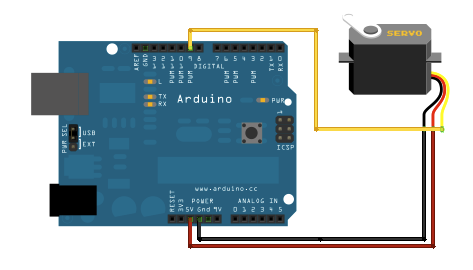
\includegraphics[width=11cm]{img/servo-circuit.png}
    \end{figure}
    
    \newpage
    
    \subsection*{%
    \cy{Shwmae!}
    \en{Code}}
    
    \begin{enumerate} %Begin numbered instructions for this section
    
    \item{
    \cy{Mae'r testun hwn yn Gymraeg.}
    \en{\textbf{Import the Servo library.}}
    
    \cy{Mae'r testun hwn yn Gymraeg.}
    \en{First we need to import a library for the Arduino, this stores some extra code so we don’t have to write as much!}
    
    \begin{lstlisting}[language=arduino,numbers=none]
    #include <Servo.h>
    \end{lstlisting}}
    
    \item{
    \cy{Mae'r testun hwn yn Gymraeg.}
    \en{\textbf{Create a servo object.}}
    
    \cy{Mae'r testun hwn yn Gymraeg.}
    \en{The first word calls the Servo library and myservo is what we will call the servo later on in the code:}
    
    \begin{lstlisting}[language=arduino,numbers=none]
    Servo myservo;
    \end{lstlisting}}
    
    \item{
    \cy{Mae'r testun hwn yn Gymraeg.}
    \en{\textbf{Create a variable to store the position of the servo.}}
    
    \cy{Mae'r testun hwn yn Gymraeg.}
    \en{We will set the servo start point as 0 for now:}
    
    \begin{lstlisting}[language=arduino,numbers=none]
    int pos = 0;
    \end{lstlisting}}
    
    \item{
    \cy{Mae'r testun hwn yn Gymraeg.}
    \en{\textbf{In setup, attach myservo to pin 11.}}
    
    \begin{lstlisting}[language=arduino,numbers=none]
    void setup() {
    myservo.attach(11);
    }
    \end{lstlisting}}
    
    \item{
    \cy{Mae'r testun hwn yn Gymraeg.}
    \en{\textbf{Move the servo.}}
    
    \cy{Mae'r testun hwn yn Gymraeg.}
    \en{The next step is to move the servo. The first part of the code is the most important part.}
    
    \cy{Mae'r testun hwn yn Gymraeg.}
    \en{Below is some pseudo code to explain what is happening.}
    
    \cy{Mae'r testun hwn yn Gymraeg.}
    \en{We start the position of the servo at 0 degrees, if the position is less than or equal to 180 degrees, then add one degree to the position variable.}
    
    \cy{Mae'r testun hwn yn Gymraeg.}
    \en{Now we have the value 1 in variable ‘pos’, myservo will move 1 degree and wait 15 milliseconds.}
    
    \cy{Mae'r testun hwn yn Gymraeg.}
    \en{Once it has moved 1 degree and waited, the code returns to the top and adds an extra degree to the position variable and loops this over and over until the position variable reaches 180.}
    
    \cy{Mae'r testun hwn yn Gymraeg.}
    \en{Once the servo reaches 180 degrees, it jumps outside the for loop, then moves along to the next for loop where it does exactly the same action but in reverse from 180 to 0.}
    
    \cy{Mae'r testun hwn yn Gymraeg.}
    \en{This can be done using the code below:}
    
    \begin{lstlisting}[language=arduino,numbers=none]
    void loop() {
      for (pos = 0; pos <= 180; pos += 1) { // goes from 0 degrees to 180 degrees
        // in steps of 1 degree
        myservo.write(pos); // tell servo to go to position in variable "pos"
        delay(15); // waits 15ms for the servo to reach the position
      }
      for (pos = 180; pos >= 0; pos -= 1) { // goes from 180 degrees to 0 degrees
        myservo.write(pos); // tell servo to go to position in variable "pos"
        delay(15); // waits 15ms for the servo to reach the position
      }
    }
    \end{lstlisting}}
    
    \end{enumerate}
    
    \newpage
    
    \section*{%
    \cy{Shwmae!}
    \en{Light Dependent Resistors Instructions}}
    
    \cy{Mae'r testun hwn yn Gymraeg.}
    \en{In order to detect the intensity of light or darkness, we use a sensor called an LDR (Light Dependent Resistor). The LDR is a special type of resistor which allows higher to pass through it (low resistance) whenever there is a high intensity of light, and passes a low voltage (high resistance) whenever it is dark.}
    
    \subsection*{%
    \cy{Shwmae!}
    \en{Hardware Required}}
    
    \begin{itemize}
    
    \item{
    \cy{Mae'r testun hwn yn Gymraeg.}
    \en{Arduino}}
    
    \item{
    \cy{Mae'r testun hwn yn Gymraeg.}
    \en{LED}}
    
    \item{
    \cy{Mae'r testun hwn yn Gymraeg.}
    \en{LDR}}
    
    \item{
    \cy{Mae'r testun hwn yn Gymraeg.}
    \en{Jumper Wires}}
    
    \item{
    \cy{Mae'r testun hwn yn Gymraeg.}
    \en{100K resistor}}
    
    \item{
    \cy{Mae'r testun hwn yn Gymraeg.}
    \en{220 ohm resistor}}
    
    \item{
    \cy{Mae'r testun hwn yn Gymraeg.}
    \en{Breadboard}}
    
    \end{itemize}
    
    \subsection*{%
    \cy{Shwmae!}
    \en{Circuit}}
    
    \cy{Mae'r testun hwn yn Gymraeg.}
    \en{You have to use a voltage divider configuration to connect the LDR. The connection diagram for the Arduino is given below, using a breadboard.}
    
    \begin{enumerate} %Begin numbered instructions for this section
    
    \item{
    \cy{Mae'r testun hwn yn Gymraeg.}
    \en{\textbf{Connect one leg of the LDR to VCC (5V) on the Arduino.}}}
    
    \item{
    \cy{Mae'r testun hwn yn Gymraeg.}
    \en{\textbf{Connect the other leg of the LDR to the analogue input pin A0 on the Arduino.}}}
    
    \item{
    \cy{Mae'r testun hwn yn Gymraeg.}
    \en{\textbf{Connect the 100K resistor to the same leg and ground.}}}
    
    \item{
    \cy{Mae'r testun hwn yn Gymraeg.}
    \en{\textbf{Connect the power/long leg of the LED straight to pin 13 on the Arduino.}}}
    
    \item{
    \cy{Mae'r testun hwn yn Gymraeg.}
    \en{\textbf{Connect the ground/short leg of the LED to the 220 ohm resistor.}}}
    
    \item{
    \cy{Mae'r testun hwn yn Gymraeg.}
    \en{\textbf{Connect the 220 ohm resistor to ground.}}}
    
    \end{enumerate}
    
    \begin{figure}[h]
    \centering
    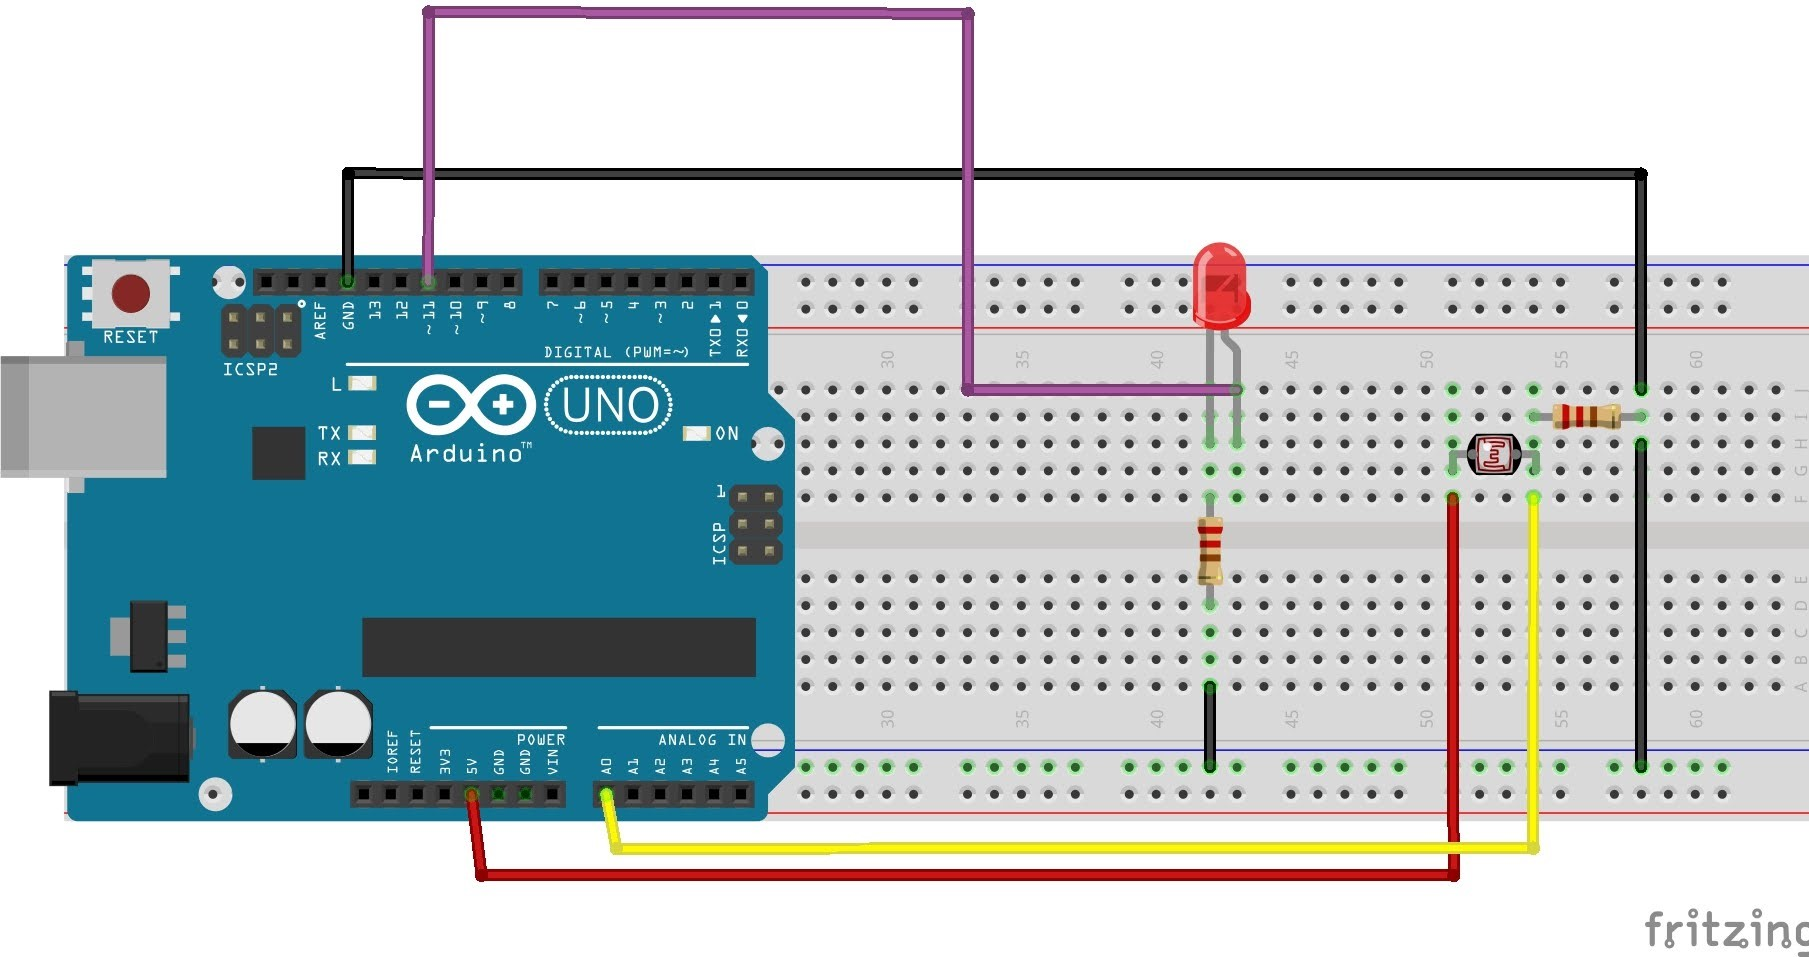
\includegraphics[width=13cm]{img/ldr-circuit.png}
    \caption*{Connecting a LDR sensor and LED to an Arduino via a bread-board}
    \end{figure}
    
    \newpage
    
    \subsection*{%
    \cy{Shwmae!}
    \en{Code}}
    
    \cy{Mae'r testun hwn yn Gymraeg.}
    \en{The first lines of code will let the Arduino know which pins are used in the code.}
    
    \begin{enumerate} %Begin numbered instructions for this section
    
    \item{
    \cy{Mae'r testun hwn yn Gymraeg.}
    \en{\textbf{Assign the pin values.}}
    
    \begin{lstlisting}[language=arduino,numbers=none]
    int LDR = A0; //LDR pin is connected to A0
    int LED = 13; //LED pin is connected to 13
    \end{lstlisting}}
    
    \item{
    \cy{Mae'r testun hwn yn Gymraeg.}
    \en{\textbf{Create a variable to store data from the LDR called LDRvalue.}}
    
    \begin{lstlisting}[language=arduino,numbers=none]
    int LDRvalue = 0; //a place to store the LDR value
    \end{lstlisting}}
    
    \item{
    \cy{Mae'r testun hwn yn Gymraeg.}
    \en{\textbf{In the setup function, begin serial communications, at 9600 bits of data per second, between your board and the computer.}}
    
    \begin{lstlisting}[language=arduino,numbers=none]
    Serial.begin(9600); //set up data connection speed
    \end{lstlisting}}
    
    \item{
    \cy{Mae'r testun hwn yn Gymraeg.}
    \en{\textbf{In the setup function, initialise the LDR as an input.}}
    
    \begin{lstlisting}[language=arduino,numbers=none]
    pinMode(LDR, INPUT); //set LDR pin (A0) as input
    \end{lstlisting}}
    
    \item{
    \cy{Mae'r testun hwn yn Gymraeg.}
    \en{\textbf{In the setup function, initialise the LED as an output.}}
    
    \begin{lstlisting}[language=arduino,numbers=none]
    pinMode(LED, OUTPUT); //set LED pin 13 as output
    \end{lstlisting}}
    
    \item{
    \cy{Mae'r testun hwn yn Gymraeg.}
    \en{\textbf{In the loop function, store values read from the analogue input in the variable LDRvalue.}}
    
    \begin{lstlisting}[language=arduino,numbers=none]
    LDRvalue = analogRead(LDR); //LDRvalue will equal values from the LDR pin
    \end{lstlisting}
    
    \cy{Mae'r testun hwn yn Gymraeg.}
    \en{Once we have the value from the LDR, we can then use it to control the brightness of the LED.}}
    
    \item{
    \cy{Mae'r testun hwn yn Gymraeg.}
    \en{\textbf{Use the value of the LDR to change the LED's brightness.}}
    
    \begin{lstlisting}[language=arduino,numbers=none]
    analogWrite(LED, LDRvalue; //LDRvalue will determine intensity of LED brightness
    \end{lstlisting}}
    
    \item{
    \cy{Mae'r testun hwn yn Gymraeg.}
    \en{\textbf{Use the serial line to print the information stored in the LDRvalue variable to the "Serial Monitor".}}
    
    \begin{lstlisting}[language=arduino,numbers=none]
    Serial.print("LDR reading is: "); //print out everything between the quotes
    Serial.println(LDRvalue); //print out data in LDRvalue
    delay(10); //delay the code for 10 milliseconds so we can keep up with the readings
    \end{lstlisting}
    
    \cy{Mae'r testun hwn yn Gymraeg.}
    \en{You should expect to see values between 0 and 1023 on teh computer when you cover and uncover the LDR. The brightness of the LED should also change slightly.}}
    
    \end{enumerate}
    
    \newpage
    
    \subsection*{%
    \cy{Shwmae!}
    \en{Example Code}}
    
    \begin{lstlisting}[language=arduino,numbers=none]
    int LDR = A0;
    int LED = 13;
    int LDRvalue = 0;
    
    void setup{
      Serial.begin(9600);
      pinMode(LDR, INPUT);
      pinMode(LED, OUTPUT);
    }
    
    void loop() { //the loop function runs over and over again forever
      LDRvalue = analogRead(LDR);
      Serial.print("LDR reading is: ");
      Serial.println(LDRvalue);
      delay(10);
    }
    \end{lstlisting}
    
    \subsection*{%
    \cy{Shwmae!}
    \en{Behaviours}}
    
    \begin{enumerate}
    
    \item{
    \cy{Mae'r testun hwn yn Gymraeg.}
    \en{Can you make the robot follow a torch?}
    
    \cy{Mae'r testun hwn yn Gymraeg.}
    \en{You may consider using “if” statements to do this.}}
    
    \end{enumerate}
    
    \newpage
    
    \section*{%
    \cy{Shwmae!}
    \en{Ultrasonic Instructions}}
    
    \cy{Mae'r testun hwn yn Gymraeg.}
    \en{This example shows you how to find the distance from an obstacle using ultrasonic sensors, for now we will return the values from the ultrasonic to the serial monitor on the Arduino.}
    
    \section*{%
    \cy{Shwmae!}
    \en{Hardware Required}}
    
    \begin{itemize}
    
    \item{
    \cy{Mae'r testun hwn yn Gymraeg.}
    \en{Arduino}}
    
    \item{
    \cy{Mae'r testun hwn yn Gymraeg.}
    \en{HC-SR04 Ultrasonic}}
    
    \item{
    \cy{Mae'r testun hwn yn Gymraeg.}
    \en{Jumper Wires}}
    
    \item{
    \cy{Mae'r testun hwn yn Gymraeg.}
    \en{Optional breadboard}}
    
    \end{itemize}
    
    \subsection*{%
    \cy{Shwmae!}
    \en{Circuit}}
    
    \cy{Mae'r testun hwn yn Gymraeg.}
    \en{Ultrasonics work by sending out pulses of sound and then counting how long it takes for those pulses to come back. So an Ultrasonic sensor actually has two parts: a transmitter and a receiver.}
    
    \cy{Mae'r testun hwn yn Gymraeg.}
    \en{If you look at the sensor it has two round bits, labelled T for transmitter and R for receiver. (In electronics things which both transmit and receive signals are often called "Transceivers" so this is really an Ultrasonic transceiver.)}
    
    \cy{Mae'r testun hwn yn Gymraeg.}
    \en{The Ultrasonic sensor has 4 wires labelled Vcc, Trig, Echo and Gnd.}
    
    \cy{Mae'r testun hwn yn Gymraeg.}
    \en{These are for the voltage, the trigger of the sonar, the echo detection signal, and the ground.}
    
    \begin{enumerate} %Begin numbered instructions for this section
    
    \item{
    \cy{Mae'r testun hwn yn Gymraeg.}
    \en{\textbf{Wire up the the first wire (voltage, or Vcc) to the 5v output of your Arduino.}}}
    
    \item{
    \cy{Mae'r testun hwn yn Gymraeg.}
    \en{\textbf{Wire up the trigger or Trig to data pin 3 on your Arduino.}}}
    
    \item{
    \cy{Mae'r testun hwn yn Gymraeg.}
    \en{\textbf{Wire up the echo detection signal to data pin 4 on your Arduino.}}}
    
    \end{enumerate}
    
    \begin{figure}[h]
    \centering
    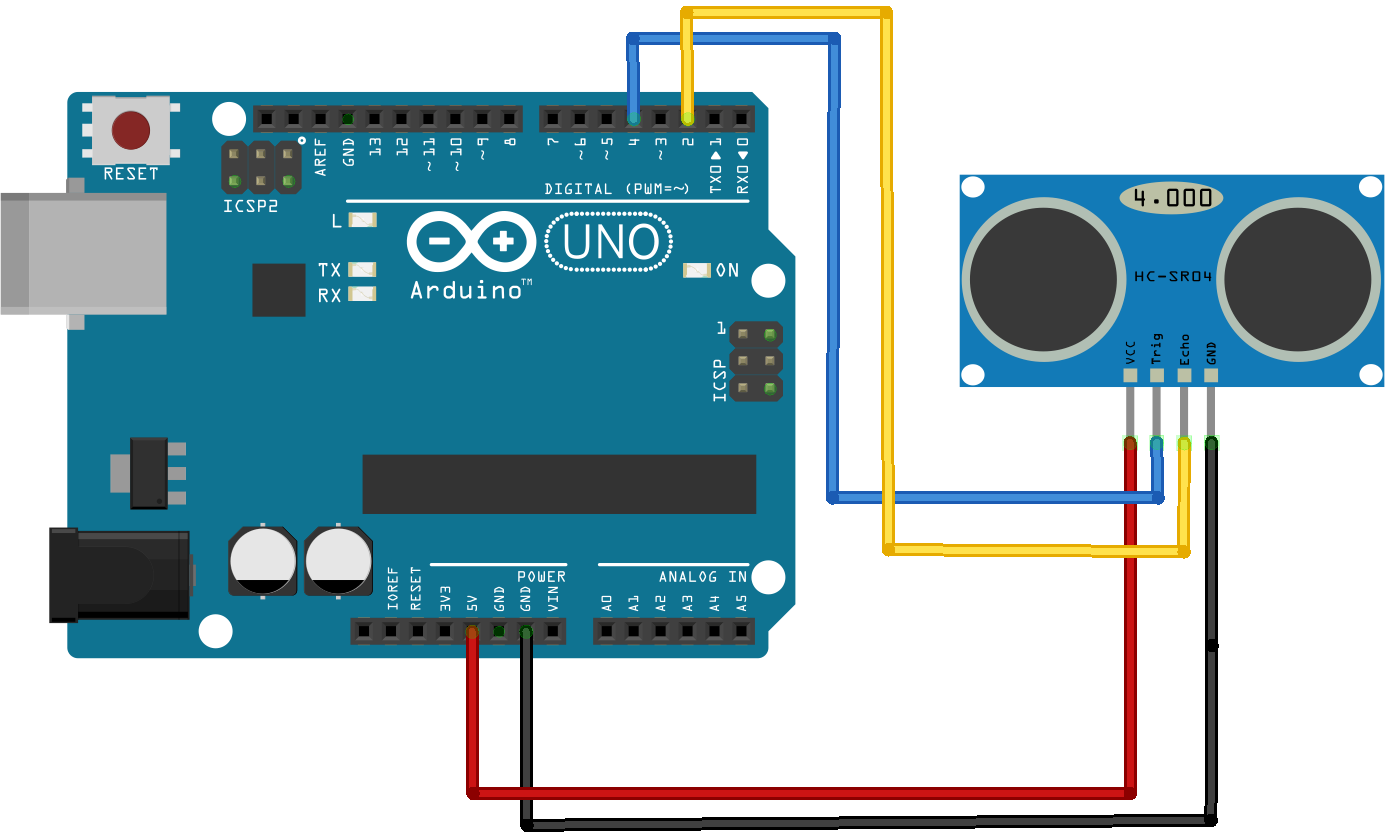
\includegraphics[width=12cm]{img/us-circuit.png}
    \caption{Connecting a Ultrasonic sensor to an Arduino}
    \end{figure}
    
    \newpage
    
    \subsection*{%
    \cy{Shwmae!}
    \en{Code}}
    
    \cy{Mae'r testun hwn yn Gymraeg.}
    \en{Remember that all Arduino programs have two parts: the setup which happens once, and is used to set up anything you need to use in the program. This is where you tell the Arduino which components are wired up to which pin, and stuff like that. There is also a loop, and the loop is repeated again and again until the Arduino is turned off (or runs out of battery power).}
    
    \cy{Mae'r testun hwn yn Gymraeg.}
    \en{In the setup function here we need to tell the Arduino which pin has the Trig connection, and which pin has the Echo connection.}
    
    \cy{Mae'r testun hwn yn Gymraeg.}
    \en{We are going to use the trigger pin to send a message to the sensor from the Arduino (so that is an OUTPUT pin), but we are going to use the Echo pin to read a message from the sensor (so that is an INPUT pin).}
    
    \begin{enumerate} %Begin numbered instructions for this section
    
    \item{
    \cy{Mae'r testun hwn yn Gymraeg.}
    \en{\textbf{Plug in your Arduino board.}}}
    
    \item{
    \cy{Mae'r testun hwn yn Gymraeg.}
    \en{\textbf{Start the Arduino Software (IDE).}}}
    
    \item{
    \cy{Mae'r testun hwn yn Gymraeg.}
    \en{\textbf{Declare the variables echo and trigger.}}
    
    \begin{lstlisting}[language=arduino,numbers=none]
    int trigger = 3;
    int echo = 4;
    \end{lstlisting}}
    
    \item{
    \cy{Mae'r testun hwn yn Gymraeg.}
    \en{\textbf{Enter the code below in the setup function.}}
    
    \begin{lstlisting}[language=arduino,numbers=none]
    Serial.begin(9600);
    pinMode(trigger, OUTPUT);
    pinMode(echo, INPUT);
    \end{lstlisting}
    
    \cy{Mae'r testun hwn yn Gymraeg.}
  	\en{As well as telling the program what's connected to what pin, it also sets up the serial monitor so we are ready to start monitoring stuff.}}
  	
  	\item{
    \cy{Mae'r testun hwn yn Gymraeg.}
    \en{\textbf{Enter the following code into the loop function.}}
    
    \begin{lstlisting}[language=arduino,numbers=none]
    long duration;
    digitalWrite(trigger, HIGH);
    delayMicroseconds(10);
    digitalWrite(trigger, LOW);
    duration = pulseIn(echo, HIGH);
    Serial.print(duration);
    Serial.println(" : duration ";
    \end{lstlisting}}
    
    \cy{Mae'r testun hwn yn Gymraeg.}
    \en{This triggers the sensor to send out a signal, then reads the signal coming back from the sensor.}
    
    \cy{Mae'r testun hwn yn Gymraeg.}
  	\en{There is a lot going on in this program.}
  	
  	\begin{itemize}
  	
  	\item{
    \cy{Mae'r testun hwn yn Gymraeg.}
    \en{First we setup a variable called duration to hold the length of time between the sound going out and the sound bouncing back.}}
    
    \item{
    \cy{Mae'r testun hwn yn Gymraeg.}
    \en{Then we trigger a quick pulse of sound (by writing HIGH to the trigger pin) - we only do this for a tiny amount of time (10 microseconds) before turning it off again by writing LOW to the trigger pin.}}
    
    \item{
    \cy{Mae'r testun hwn yn Gymraeg.}
    \en{We then capture the time from the pulse being sent out to coming back by looking for a HIGH pulseIn on the echo pin.}}
    
    \item{
    \cy{Mae'r testun hwn yn Gymraeg.}
    \en{Finally we print the duration out to the serial monitor.}}
    
    \end{itemize}
    
    \newpage
        
    \item{
    \cy{Mae'r testun hwn yn Gymraeg.}
    \en{\textbf{Test the program by clicking the tick.}}}
    
    \item{
    \cy{Mae'r testun hwn yn Gymraeg.}
    \en{\textbf{Put the program on the Arduino using the arrow button.}}}
    
    \item{
    \cy{Mae'r testun hwn yn Gymraeg.}
    \en{\textbf{Open the serial monitor.}}
    
    \cy{Mae'r testun hwn yn Gymraeg.}
    \en{To open the serial monitor, click on the button that looks a bit like a magnifying glass in the top right corner of the Arduino IDE window (it will say "Serial Monitor" when you hover over it). That will open up a new window which contains the stuff you have printed to Serial. You should see something like this:}
    
    \begin{lstlisting}[language=arduino,numbers=none]
    386: duration
    417: duration
    381: duration
    \end{lstlisting}
    
    \cy{Mae'r testun hwn yn Gymraeg.}
    \en{These are measurements of how long it took (in microseconds) for the sound to bounce off a thing in the world and then back to the ultrasonic sensor.}}
    
    \end{enumerate}
    
    \subsection*{%
    \cy{Shwmae!}
    \en{Going from a measurement of time to a measurement of distance}}
    
    
    \begin{enumerate} %Begin numbered instructions for this section
    
    \item{
    \cy{Mae'r testun hwn yn Gymraeg.}
    \en{\textbf{Set up a barrier near your computer, and get hold of a ruler.}}}
    
    \item{
    \cy{Mae'r testun hwn yn Gymraeg.}
    \en{\textbf{Measure the distance from the sensor to the barrier, and fill in a table of measurements from the serial monitor.}}}
    
    \begin{enumerate} %Begin numbered instructions for this section
    
    \item{
    \cy{Mae'r testun hwn yn Gymraeg.}
    \en{If the barrier is 10cm from the sensor, how long does it take the sound to travel?}}
    
    \item{
    \cy{Mae'r testun hwn yn Gymraeg.}
    \en{Take some more measurements. Can you come up with a way of converting ``sound-travel-time'' into centimetres?}}
    
    \item{
    \cy{Mae'r testun hwn yn Gymraeg.}
    \en{If you can come up with a useful conversion system, can you then get that into your program - that is, can you work out how to get your program to give an output in centimetres? Give it a go, and then test your ultrasonic ruler against a real ruler.}}
    
    \end{enumerate}
    \end{enumerate}
    
    \subsection*{
    \cy{Shwmae!}
    \en{Behaviours}}
    
    
    \begin{enumerate}
    
    \item{
    \cy{Mae'r testun hwn yn Gymraeg.}
    \en{Can you avoid obstacles using the ultraonic sensor whilst the robot is driving?}}
    
    \end{enumerate}

    \end{document}